\documentclass{standalone}
\usepackage{tikz}
\begin{document}
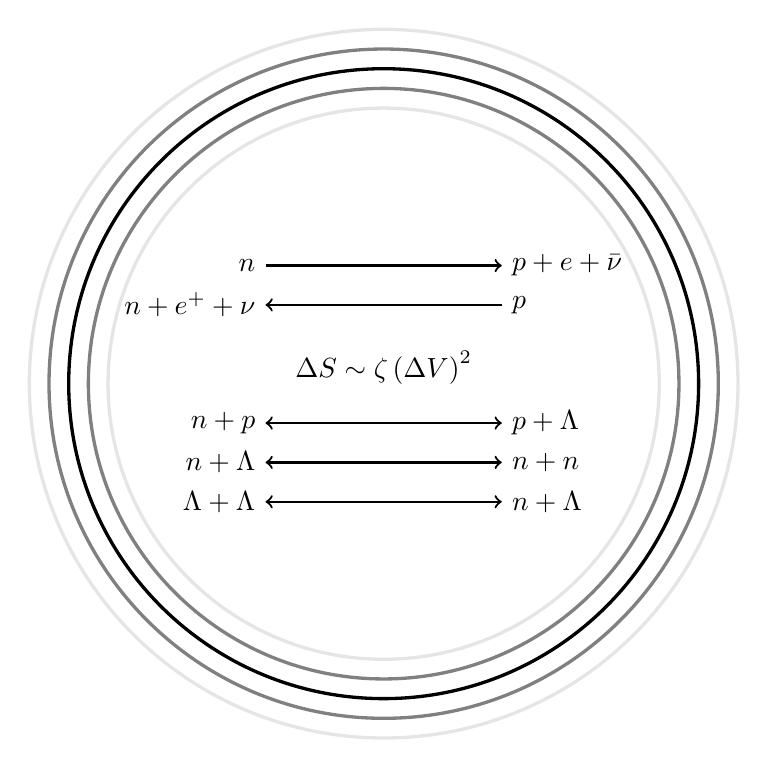
\begin{tikzpicture}
    \draw[very thick](0,0) circle (4);
    \draw[color=black!50, very thick](0,0) circle (3.75);
    \draw[color=black!10, very thick](0,0) circle (3.5);
    \draw[color=black!50, very thick](0,0) circle (4.25);
    \draw[color=black!10, very thick](0,0) circle (4.5);
    \draw[thick, ->] (-1.5,1.5) node[left]{$n$}  -- ( 1.5,1.5) node[right]{$p+e+\bar{\nu}$};
    \draw[thick, ->] ( 1.5,1)   node[right]{$p$} -- (-1.5,1) node[left]{$n+e^++\nu$};
    \draw[thick,<->] (-1.5,-0.5) node[left]{$n+p$}  -- ( 1.5,-0.5) node[right]{$p+\Lambda$};
    \draw[thick,<->] ( 1.5,-1) node[right]{$n+n$} -- (-1.5,-1) node[left]{$n+\Lambda$};
    \draw[thick,<->] ( 1.5,-1.5) node[right]{$n+\Lambda$} -- (-1.5,-1.5) node[left]{$\Lambda+\Lambda$};
    \node[] at (0,0.2) {$\Delta S \sim \zeta \left(\Delta V\right)^2$};
    \end{tikzpicture}
\end{document}

